%--------------------------------------------------
\subsection{Literature and Operational Setting}

\subsubsection{Academic Literature}
This work does not launch neatly from a single `conversation' \citep{Booth:2009vy} in the scientific literature.  Rather, it is motivated by problems arising in a practical forecast setting and will respond to conversations across multiple sub-disciplines.  The very fact that ocean forecasting contains such distinct specialisations is relevant and is discussed below in \ref{S:two_perspectives}.\\
Also worthy of comment is the fact that the literature addressing ocean tides is especially long and vast.  Only a subset of this tradition will be considered directly relevant to the present work; primarily that addressing formulations of ocean tidal analysis and prediction.  



%--------------------------------------------------
%\subsection{Operational Forecast Setting.}  
\subsubsection{Operations}
\label{S:operational_setting}
It is necessary for the present review scope to extend a little beyond the academic literature itself to include the operational setting. Operational considerations are fundamental to the motivation and methods behind this research.



Operational centres such as the \BOM{} routinely provide oceanographic forecasts.  Although often contentions as to a strict definition, \emph{operational} in an agency context implies that forecasts are produced in a regular and reliable manner for general promulgation.\\
Ocean forecasts produced by an operational centre represent an instance of \emph{operational oceanography}.  This generic neologism is increasingly associated with activities that involve rapid dissemination of ocean data; but the pertinent connection with \GODAE{} is discussed further below in Section\ref{S:operational_oceanography}.\\



Levels of documentation regarding operational forecasts often fall far behind aspirations and many details are only retrained in institutional practices and assumptions.  This is especially the case with regard to harmonic tide prediction.  \\
Operational manuals and handbooks exist to codify aspects of coastal sea level observations, technology and transmission - eg \citep{IOC:2005tj}, \citep{Level:2011wu}, Canada, \citep{Parker:2007wq}.  However, analysis methods and design justifications are much less formally documented, if at all.  The International Oceanographic Commission understates this situation simply:
\begin{quote}
many organizations have developed their own method of tidal analysis. \citep{IOC:2005tj}
\end{quote}

Expectations about sea level forecasts have largely been defined by harmonic tidal prediction practice.  
%For instance, tide predictions are ubiquitously delivered without any quantification of error.  Tide tables are typically issued for at least one year in advance and many marine users are legally required to carry the official tables.  In this regard, official harmonic predictions are just as much a \emph{declaration} as a forecast.  More so, in that tidal component of sea level is not directly observable and that different authorities do not produce identical forecasts. \\




Somewhat distinct from international forecast centres, the \BOM scope spans a vast mainly contiguous coastline; much of which is sparsely populated and under-observed.  Around that vast coastline other regional authorities engage in activities that overlap with or transform the outputs of the national agency.  For instance, regional agencies such as Manly Hydraulics Labratory in NSW perform their own harmonic analysis and issue tide tables.   %Agencies such as the State Emergency Service in Victoria rely on national forecast products in responding to extraordinary coastal sea level events.

\subsubsection{Other Sea Level Forecasts}  
Whilst this document is limited to sea level forecasts within bounds defined above, the operational centre produces a variety of `sea level' forecasts in a broader sense.  All involve elevation of the ocean interface but inter-compatablity is not always clear nor necessarily relevant.  \\
The following list is illustrative:
\begin{inparaenum}[(a)]
\item \underline{tidal predictions}; %produced annually for port locations using conventional harmonic analysis;
\item gridded \underline{sea level anomaly} forecasts; %produced daily using an \OGCM{}-based system; 
\item gridded \underline{wind-wave} forecasts; % produced at twice-daily and representing a particular range of sea level variations with directional spectra; 
\item \underline{estuarine river level} forecasts; % produced on an event basis using a linear catchment-runoff model; 
\item tropical cyclone \underline{storm surge} forecasts; % produced on an event basis using a variety of parametric and gridded systems;
\item coastal zone \underline{tsunami} warnings ;%using a precomputed set of gridded model scenarios;
\item gridded \underline{seasonal} outlook sea level anomaly forecasts;
\end{inparaenum}




\subsubsection{Requirements of Operational Forecasts}  
Operational centres are different to research organisations and have specific requirements. Appropriate forecast approaches prioritise the following qualities:
\begin{enumerate}
\item \underline{Robustness}: Resilience to withstand and promptly recover from a broad range of impacts is paramount to an operational system.  Inevitable operational disturbances (such as corrupt inputs, missing inputs, hardware failures and human error) are a fundamental design consideration.
\item \underline{Routine Operability}:  Realistic implementation within the day-to-day workings of an operational centre places a high value on simplicity, automation and maintainability .
\item \underline{Predictive skill}:  Forecasts only have value in as much as they provide meaningful `environmental intelligence' regarding the future \cite{BureauofMeterology:2010tq}.
\item \underline{Universalism}/generic applicability/scalability:  An operational centre will not prioritise systems that are highly peculiar to any one location or that require large investments in local tailoring.
\end{enumerate}



Operational considerations like these have influenced sea level science more broadly.   But the details of these pragmatic constraints have changed historically; notably with regard to computing, observing and communications technology.\\
Consider for instance how Doodson's \citep{Doodson:1928wf} tidal procedures reflect the practical limits imposed by human computers applying cut-out stencils upon paper records.  Furthermore, this scientific window into sea level fundamentally relies on routine observation procedures of port authorities.  Looking forward, developments in remote observation technology such as wide-swath altimetry (eg \citep{Ray:2011tj}) promise to open a new perspective on sea level and subsequently on operational ocean prediction. \\


\subsubsection{Organisational Culture}
In contrast to the promises of technical advance and the proverbial `next' satellite platform, an important characteristic of the operational  setting is a cultural requirement for continuity and organisational inertia.  Operational centres are risk adverse with regard to system change.  \\
It is noteworthy that tidal forecasts are typically issued by a dedicated department (or an entirely different organisation), quite separate from that maintaining the newer dynamical ocean systems.\\



%--------------------------------------------------
\subsection{Two Broadly Different Forecasting Perspectives} 
\label{S:two_perspectives}
\subsubsection{Relevance of History}
A historical perspective is required to understand how \emph{operationally forecasting} sea level has raised problems that are both practical and academic in nature; including issues of terminology.\\
The literature surrounding \OGCM{}'s is in practice world apart from routine tidal analysis.  The respective motivations and vocabulary are not entirely compatible.  Despite the differences however, both are now ultimately providing sea level forecast information within operational centres.  




Tidal harmonic methods have for many decades provided the only routine source of sea level forecast - and with great success.  In contrast, time stepping primitive equation dynamic models and data assimilation are relatively new arrivals to operational centres.  These represent two qualitatively different perspectives on sea level prediction and form distinct sub-disciplines of oceanography.\\


\subsubsection{Intersection of Approaches}
Over the past decade, the operational evolution of \OGCM-based prediction has increasingly brought these approaches into the same space and highlighted what could be called `border issues' or something akin to Gallison's `trading zone' \citep{Galison:1996uc}.  A fuzzy border exists as these nominally separate schools of practice are in fact not mutual exclusive with regard to neither the physical phenomenon being modelled nor forecast product outputs.\\
Most evidently to date, issues have arisen with regard to interpreting and communicating nominally `nontidal' forecasts in light of existing harmonic tide predictions.   Directions in the ongoing development of \BL{} and similar systems promise only to increase the amount of overlap into the previously independent practices of harmonic analysis eg \cite{Arbic:2010us}\\
Here Munk and Cartwright's aphorism from the 1960's regarding tidal analysis is illustrative:
\begin{quote}
\dots predicting and learning are in a sense orthogonal, and the most interesting effects are those that cause the most trouble with a forecasting: the continuum, the nongravitational tides, and the non-linear interactions.\citep{Munk:1966ts} 
\end{quote}
Forecasts from \BL{} and other similar systems now represent sea level attributable to exactly these troublesome areas; or at least some physical subset therein.  By doing so, these relatively new ocean forecast capabilities invite deeper understanding of the relationship with tide prediction. 



It is illustrative that Jayne refers to ``vexing problems'' \citep[pp812]{Jayne:2001tr} arising from applying frequency-domain theory in time-domain numerical tide modelling.


\begin{figure}[h]
\begin{center}
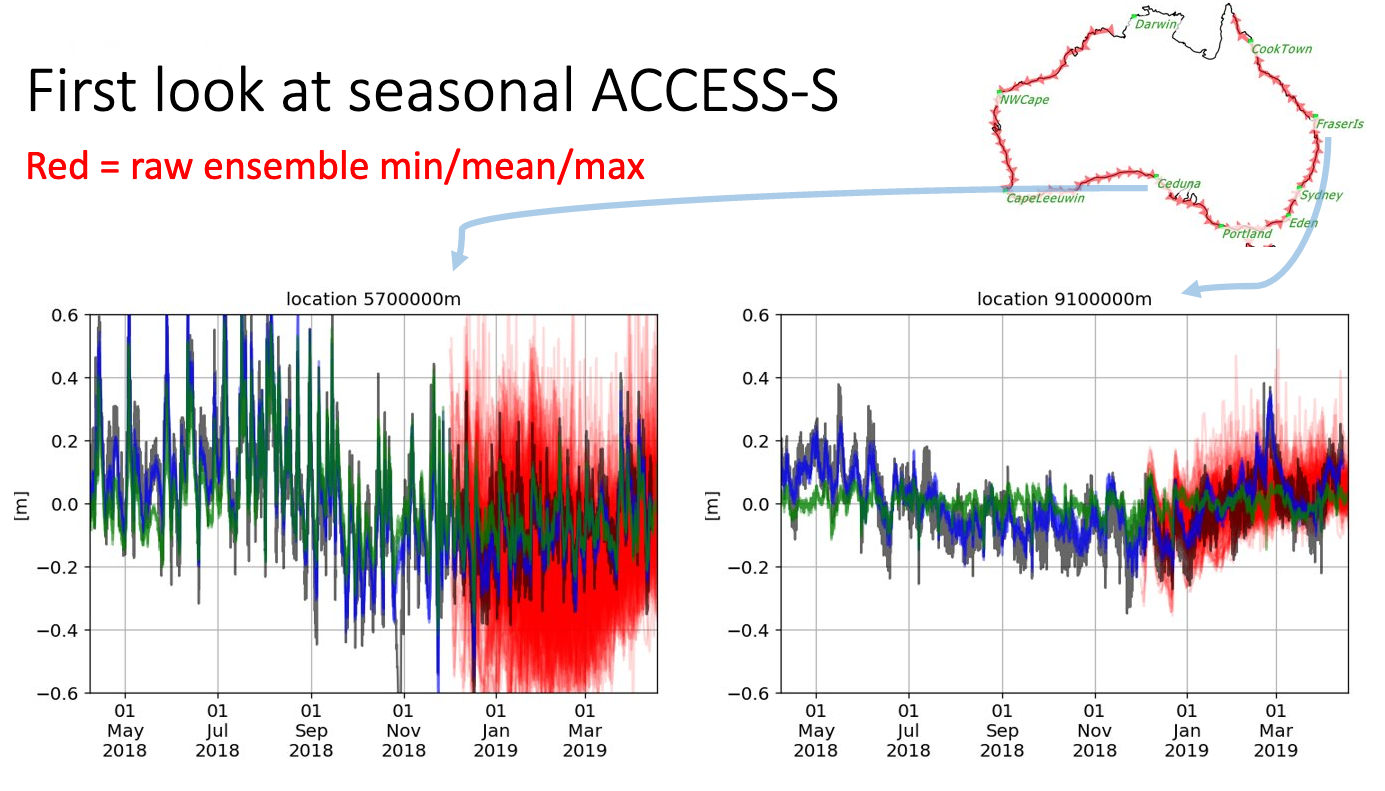
\includegraphics[width=120mm]{figures_2/spectra_cartoon_1.png}
\caption{Conventional decomposition concept: mixed sea level spectra comprising discrete tidal `lines' and red turbulent continuum.  Implementation of this concept has ramifications for sea level forecasting.}
\label{fig:SPECTRA_CARTOON}
\end{center}
\end{figure}


\subsubsection{Characterisation as Tidal and Nontidal}

\BoxBegin
Prima facie, the two perspectives are represented by the conceptual decomposition of sea level into \underline{nontidal} and \underline{tidal} signals;  the dynamic continuum and harmonic lines illustrated in Figure \ref{fig:SPECTRA_CARTOON}.  Whilst the decomposition concept is problematic, it is still a useful base from which to launch the present discussions.   
\BoxEnd


The historical approach of Gallison's \citep{Galison:1987wh} provides a template to understanding the situation with sea level forecasting.  Gallison asserts that in modern scientific culture, apparent mismatches between different sub-disciplines are not necessarily cause for concern and are in fact the norm.  His description of physics as `neither unified nor splintered into isolated fragments' \citep[pp 782]{Galison:1987wh} also appears apt for operational sea level forecasting.  Thus also is Peterson's assertion of `...the fundamental plurality of factual claims, methodologies, and epistemic values in scientific practice' \cite{Petersen:2012tr}.  Viewing sea level as a stationary set of harmonics is at face value quite at odds with a view of the ocean as a turbulent fluid.\\
But the respective strengths of these ostensibly incompatible views does invite closer examination. \\
Thus the present thesis is situated in a type of scientific `trading zone' between the perspectives of tidal analysis and \OGCM{}-based ocean prediction, sharing a common ground in the routine forecasting of sea level at similar time/length scales.\\



It is emphasised that this historical characterisation of sea level prediction as two broadly separate schools should not be regarded as a simple story of Old versus New.  On the contrary, the intention here is to emphasise how historical factors contribute to framing of the present research and to facilitate clear discussion of the subject matter.






%--------------------------------------------------

\subsection{Operational Oceanography}
\label{S:operational_oceanography}


In contrast to the existence of operational centres, `Operational Oceanography' is a relatively recent neologism that, as with much of the terminology under consideration here, leaves some room for interpretation as to what exactly it designates.
\begin{quote}
Operational Oceanography can be defined as the activity of systematic and long-term routine measurements of the seas and oceans and atmosphere, and their rapid interpretation and dissemination.\citep{EuroGOOS:ws}
\end{quote}
Beyond the very inclusive definition given above, this term in current use strongly implies a role for real-time communications, the involvement of numerical modelling of some form and the provision of a sustained service e.g. \citep{Flather:2000ju}.   For present purposes, operational oceanography designates an approach to ocean forecasting that is fundamentally based in numerical modelling and data assimilation.  However it is noted that the designation is also being used to retrospectively encompass pre-existing ocean service provision by government agencies: for instance the recent placement of tidal services within NOAA's Center for Operational Oceanographic Products and Services \citep{NOAA:wv}.




The Global Ocean Data Assimilation Experiment \GODAE{} \citep{Bell:2009uv} serves as a historical reference point for the evolution of \OGCM{}-based ocean prediction systems such as \BL{}.  The \GODAE{} heritage can be seen as an instance of `big science' \citep{Petersen:2012tr} in the sense that it fundamentally relies on the coordination of large organisations, global observation and communications networks and the maintenance of expensive physical assets.   This tradition of ocean prediction is very directly related to the more mature development of atmospheric numerical weather prediction (\NWP).  
\begin{quote}
The central idea of GODAE - to demonstrate the feasibility and utility of real-time, global ocean forecasting - was based on the experiences of the meteorological community in the First Global Atmospheric Research Program Global Experiment, known as FGGE. \citep{Bell:2009uv}
\end{quote}



%-----------------%
\subsubsection{Ocean General Circulation Models}

Like \NWP, the term Ocean General Circulation Model (\OGCM{}) implies a certain class of geophysical fluid simulation.  \OGCM{}s simulate temporal evolution of the physical ocean state by means of time-stepped integration of a discretised set of fluid dynamic equations.  Such models embody numerical methods applied to a mixed boundary condition/initial condition constrained set of partial differential equations  \citep{Griffies:2004vs}.  An \OGCM{} is thus a specialised instance of the application of Computational Fluid Dynamics.\\



As with computational fluid dynamics more generally, a distinction between \emph{resolved} and \emph{unresolved} scales is paramount.   
\begin{quotation}
\noindent
Oceanic flow is generally nonlinear, chaotic and turbulent.  Correspondingly, the ocean's spatial and temporal scales are extremely broad\dots{}.  Coupling occurs between the scales due to nonlinear cascades of flow properties, such as energy and tracer variance.  Furthermore, it is not possible to measure every spatial point with a fluid, for all time instances.  These practical limitations restrict access to information about the turbulent fluid's spatial and temporal properties.  Sensitive dependence on initial conditions in this turbulent flow then severely limits predictive capabilities.  This lack of information and limited predictability motivates a formulation of averaged or mean field fluid equations.\citep[Sec 2.5]{Griffies:2004vs}
\end{quotation}
The presence of information cascades between scales in a turbulent fluid requires a simulation to somehow account for the dynamic exchanges between resolved and unresolved scales.  Such effects are incorporated into a numerical simulation by means of parameterisations of sub-grid scale (SGS) dynamics.\\
Griffies suggests that an \OGCM{} then can be conceived of as simulating some type of averaged motion over an infinite ensemble of hypothetical ocean realisations.  The imagined spread amongst this ensemble then is proportional to  the scales allocated to the SGS parameterisations.
Alternatively, Stevens casts \OGCM{}s into the class of geophysical `pseudofluid' simulations \citep{Stevens:2001kb}.   Geophysical turbulence drives a pragmatic requirement for SGS parameterisation, described as the simulation of a pragmatically `aggregated' model system.   Whatever the characterisation, SGS parameterisations are fundamental to the meaning and interpretation of \OGCM{}s.   Subsequently comparison of the simulated pseudeofluid with observational data is prone to interpretational nuance and are ``too often ad hoc, uncritical, and/or irrelevant''\citep[pp 286]{Stevens:2001kb}.   Such issues will be addressed in the body of this research with regard to evaluation and data assimilation.\\

\begin{figure}[h]
\begin{center}
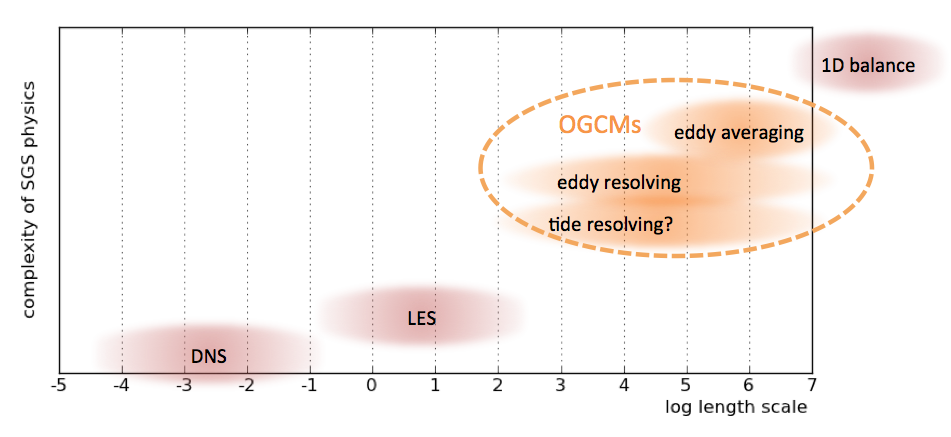
\includegraphics[width=120mm]{figures_2/model_types_schematic.png}
\caption{Schematic illustration of place of \OGCM{}s in terms of SGS parameterisation of the broad scale range of a turbulent ocean.  For reference, methods from turbulence studies are included: Direct Numerical Simulation and Large Eddy Simulation. Following \citep[fig 5.2]{Petersen:2012tr} and \citep{Stevens:2001kb}.  Inclusion of explicit tides is tentatively placed as a reduction of parameterisation without increased spatial scale resolution.}
\label{fig:models}
\end{center}
\end{figure}


An \OGCM{} is at core a method of time-stepping an averaged form of the Navier-Stokes equations with a specialised configuration. The ocean is viewed as a turbulent fluid and simulated with a relatively high degree of aggregation, implemented via a range of SGS parameterisations.\\
Figure \ref{fig:models} schematically lays out broad classes of computational fluid models with regard to resolved scales and complexity of SGS parameterisation.  In general, numerical SGS parameterisations need to be adjusted to suit the spatial resolution of a model - parameterisations do not generally scale.
Some common features to all \OGCM{}s are the following:
\begin{itemize}
\item distinction of vertical and horizontal dimensions;
\item very flat aspect ratios;
\item separate semi-empirical parameterisations for horizontal and vertical processes and turbulent closure schemes;
\item exclusion of specific classes of dynamics - eg. acoustic waves, tidal forcing, 
\end{itemize}



From an organisational perspective, a contemporary \OGCM{} embodies a large amount of collective and accumulated programming effort in many lines of computer code; too much for any one person to understand in detail.  This is a common situation in modern `big science' simulation practice \citep{Petersen:2012tr}. \\




%-------------------------------

\subsubsection{\BL{} and \MOM{}}
Whilst a range of operational \OGCM{}s exist, the present study will be intentionally limited to model(s) considered directly relevant to the \BOM{}.   Fundamentally this involves the community code `Modular Ocean Model' \MOM{} \citep{Griffies:2008vh}.  The configuration of \MOM{} named \OFAM{} forms the \OGCM{} component of \BL{} \cite{Brassington:2012wm}.  \MOM{} versions 4.1 and 5 are thus specifically within this scope.\\
\MOM{}  employs a finite-difference method on a structured horizontal grid.  Whilst \MOM{} supports generalised vertical coordinate choices, the \OFAM{} configuration implements a depth-based coordinate with a free-surface.  Further details of configuration will be addressed where relevant in the body of this research.\\
In response to contemporaneous operational developments within the \BOM{}, the possible relevance of \ROMS{} \cite{Shchepetkin:2005eh} to coastal sea level forecasts is flagged as potentially presenting future insights to the present research.


In contrast, global \emph{tide} models represent a very distinct class of numerical representation of the ocean.  Whilst sharing some characteristics, these models are fundamentally different to \OGCM{}s and are discussed below in Section \ref{S:TIDE}.

%-----------------%
\subsubsection{Ocean Observations and Data Assimilation}
Neither models nor observations can provide forecast value in isolation.   \\




Data assimilation is fundamental to rendering an \OGCM{} relevant to operational forecasts.  Data assimilation is the framework for meaningfully combining recent ocean observations and the chaotic dynamics embodied by an \OGCM{}.\\
Ocean data assimilation can be seen as a technical implementation of Baye's Theorem, in that it involves the `optimal utilisation of information from difference sources' \citep{Zaron:2011ft}.\\



Operational oceanography is enabled by reliable ongoing data delivery from the composite global ocean observing system.  \\
Viewed as a whole, the composite array of routine ocean observations is referred to as the `Global Ocean Observing System' \GOOS{} \citep{Komen:1999ch}.  The \GOOS{}    includes satellite-based earth observations and insitu platforms such as Argo.  It is noted that \GOOS{} was also formalised as an international entity under the auspices of the United Nation in 2005 \citep{IOC:2005wv}.\\
Whilst quantitative observations have expanded massively in recent decades,  the ocean is fundamentally under-observed for the purposes of state estimation. Despite the apparently huge data volumes the \GOOS{} provides a set of data that is very sparse relative to the degrees of freedom of the physical ocean state.\\




\subsubsection{Significance of Altimetry}
Satellite-based ocean altimetry provides a data stream of special significance to contemporary ocean forecasting \citep{Fu:2001ub}. \\


A series of satellite platforms have now provided along-track nadir looking measurements of ocean topography for over 20 years \citep{Wilson:2010hy}.   It is remarkable and fortunate that much of this cumulative time coverage is due to beyond-design-life operation. \\

Derivation of sea level quantities from satellite mounted radar instruments requires many intermediate data sources and estimates. Such a derivation is particularly challenging in shallow water and near coastal boundaries \citep{Woodworth:2011bf} and for this reason altimetry has primarily been considered an open-ocean data source.   Amongst diverse applications, these data have directly enabled developments in explaining open ocean tides (eg.\citet{Egbert:1996vr},  \citet{Lefevre:2011dg}) and mesoscale ocean variability (eg.  \citet{Wunsch:1998bq}, \citet{Chelton:vi}). \\
It is relevant to again highlight that historically tidal and nontidal uses of altimetry have formed distinct sub-disciplines in the literature.   The separation is directly analogous to the situation with regard to tide gauge data.  These different perspectives on the observations have been mutually complementary; facilitating the decomposition of sea level into tidal/nontidal sub-signals.    The present research will require close consideration of the nature of this split with regard to ocean forecasting.\\
Although the importance of assimilating altimetry data into ocean models is common to the tidal and nontidal perspectives, implementations contain some stark contrasts.  This simply reflects the fundamental difference between viewing the ocean as a turbulent fluid evolving in time, or viewing it as a stationary spectral field.
 
